% CONVENTIONS
% British English: Behaviour, maximisation etc
% alphabetical ordering of packages (if possible, exception i.a. hyperref) -> quicker search
% low/high probabilities instead of small/large

\documentclass[%
	11pt,
	abstract=true,	
% 	captions=figureheading,
% 	numbers=noenddot,
	bibliography=oldstyle					% more compact
]{scrartcl}

% \documentclass[11pt]{article}
%\documentclass[12pt]{article}
%\documentclass[12pt,a4paper]{article}

\usepackage[UKenglish]{babel}
%\usepackage[cmbold]{mathtime}
%\usepackage{mt11p}
% \usepackage[blocks,auth-sc-lg,affil-it]{authblk}
\usepackage{amsfonts}
\usepackage{amssymb}
\usepackage{amsthm}
\usepackage{array}
\usepackage{booktabs}
%\usepackage{breakurl}
%\usepackage{breakurl}
\usepackage{caption}
%\usepackage[justification=centering]{caption}
%\captionsetup[table]{format=plain,labelformat=simple,labelsep=period,singlelinecheck=true}%
\usepackage{comment}
\usepackage{dcolumn}
\usepackage{enumitem}
\usepackage{epigraph}
\usepackage{epsfig}
\usepackage{epstopdf}
%\usepackage{eurosym}
\usepackage{float}
\usepackage{footmisc}
\usepackage{geometry}
% \geometry{left=3cm,right=2cm,bottom=4cm,top=3cm}
% \geometry{left=1.25in,right=1.25in,top=1.25in,bottom=1.25in}
% \geometry{left=1in,right=1in,top=1in,bottom=1in}
\usepackage{graphicx}			% automatically \usepackage{graphics}
%\usepackage[misc]{ifsym}
\usepackage{listings}
\usepackage{makecell}
\usepackage{mathrsfs}
\usepackage{mathtools}		% superset of amsmath
\usepackage{marvosym}
% \usepackage[round]{natbib}
%	\bibliographystyle{unsrtnat}
% \bibliographystyle{ecta}
\usepackage{multirow}
\usepackage{nicefrac}
\usepackage[percent]{overpic}
\usepackage{pdflscape}
\usepackage{pgfplots}							% loads xcolor
\usepackage{placeins}
\usepackage{rotating,tabularx}
%\usepackage[graphicx]{realboxes}
\usepackage{setspace}
\usepackage{subcaption}							% for subfigure & -captions [better than package subfig(ure)]
% \usepackage{subfigure}
\usepackage[decimalsymbol={.},exponent-product=\cdot,group-separator={,}]{siunitx}	% nice formatting of units, digit grouping, etc. 
\usepackage{threeparttable}
\usepackage{tikz}																% loads xcolor
\def\checkmark{\tikz\fill[scale=0.4](0,.35) -- (.25,0) -- (1,.7) -- (.25,.15) -- cycle;}
%\usetikzlibrary{snakes}
%\usetikzlibrary{patterns}
\usetikzlibrary{decorations.pathreplacing}
%\def\checkmark{\tikz\fill[scale=0.4](0,.35) -- (.25,0) -- (1,.7) -- (.25,.15) -- cycle;}
\usepackage[normalem]{ulem}					% no underline instead of emphasis/italic
\usepackage{xspace}

%%%%%%%%%%%%%%%%%%%%%%%%%%%%%%%%%%%%%%%%%%%%%%%%%%%%%%%%%%%%%%%
%%%%%%%%%%%%%%%%%%%   HYPERREF		%%%%%%%%%%%%%%%%%%%%%%%%%%%%%
%%%%%%%%%%%%%%%%%%%%%%%%%%%%%%%%%%%%%%%%%%%%%%%%%%%%%%%%%%%%%%%

\usepackage[
% 	dvipdfm,
%   pdftex,
%   bookmarksopen,
%   bookmarksopenlevel={2},
%   bookmarksnumbered=true,
 	breaklinks=true,
 	urlcolor=blue,															% affects DOIs & URLs
  colorlinks=true,
  linkcolor=blue,
  citecolor=blue,
%   hyperfootnotes=false,
% 	linktocpage=true,
%   pdfstartview=FitB,
%   pdfpagelayout = SinglePage,
%   pdfview=FitH,
%   pdfcenterwindow = false
%   pdfpagemode = FullScreen
]{hyperref}
\usepackage{url,doi} 											% !! load after hyperref (colouring issues)
% \usepackage{showlabels}										% !! load after amsmath, hyperref

\hypersetup{
pdfauthor={Ole Peters, Alexander Adamou, Yonatan Berman, Mark Kirstein},
pdftitle={What are we weighting?},
pdfsubject={See abstract},
% pdfsubject={ECTA Submission},
pdfkeywords={Decision Theory, Prospect Theory, Probability Weighting, Ergodicity Economics}
% colorlinks,
% linkcolor={blue!50!black},
% citecolor={blue!50!black},
% urlcolor={blue!50!black}
}

%%%%%%%%%%%%%%%%%%%%%%%%%%%%%%%%%%%%%%%%%%%%%%%%%%%%%%%%%%%%%%%
%%%%%%%%%%%%%%%%%%%%%%%   CAPTION FORMAT   %%%%%%%%%%%%%%%%%%%%
%%%%%%%%%%%%%%%%%%%%%%%%%%%%%%%%%%%%%%%%%%%%%%%%%%%%%%%%%%%%%%%
% \setkomafont{caption}{\sffamily}										%  Caption-Formatierung
\setkomafont{captionlabel}{\sffamily\bfseries}
\setcapindent{1em}

%%%%%%%%%%%%%%%%%%%%%%%%%%%%%%%%%%%%%%%%%%%%%%%%%%%%%%%%%%%%%%%
%%%%%%%%%%%%%%%%   BibLateX w/ BibTeX(8)   %%%%%%%%%%%%%%%%%%%%
%%%%%%%%%%%%%%%%%%%%%%%%%%%%%%%%%%%%%%%%%%%%%%%%%%%%%%%%%%%%%%%
\usepackage[
arxiv=abs,																					% Link to arXiv abstract page
autocite=footnote,																		% structur of \autocite{key}
autolang=hyphen,																		% active if langid is set
% autopunct=false,																	%
backend=bibtex,
% backend=bibtex8,																		% Backend choice BibTeX8 case-sensitive sorting 
backref=true,																				% page cited in the paper
% bibencoding=latin1,
bibstyle=authoryear,																% style in bibliography
% bibstyle=draft,																		% style in bibliography
% bibwarn=true,
citestyle=authoryear-comp,													% style in the document
dashed=false,																				% always repeat author names in bibliography
% -- hyperref=true,																		%
% language=autobib,																		% bibliography language same as language of origin
% sortcites=true,																			% sort citations in the text
sortcites=false,																		% do not sort citations in the text
% sorting=nyt,																				% sorting in bibliography
maxbibnames=11,																			% limit authors in bibliography to 11
maxcitenames=2,																			% start to use et alii
% minbibnames=10																			% Angabe wie vieler Autoren nach Schnitt
mincitenames=1,																			% cut to X authors with et al.
url=true,doi=true,eprint=true,											% print url,doi,eprint
useprefix=true,																			% consider nobiliary particle von, van, de, etc.
]{biblatex}

\addbibresource{../LML_bibliography/bibliography}

%%%%%%%%%%%%%%%%%%%%%%%%%%%%%%%%%%%%%%%%%%%%%%%%%%%%%%%%%%%%%%%
%%%%%%%%%%%%%   STYLE OF THE REFERENCES   %%%%%%%%%%%%%%%%%%%%%
%%%%%%%%%%%%%%%%%%%%%%%%%%%%%%%%%%%%%%%%%%%%%%%%%%%%%%%%%%%%%%%

\newcommand*\person[1]{\textsc{#1}}									% prints author names as small caps
\renewcommand{\mkbibnamegiven}[1]{\person{#1}}
\renewcommand{\mkbibnamefamily}[1]{\person{#1}}
\renewcommand{\mkbibnameprefix}[1]{\person{#1}}
% \renewcommand{\mkbibnamesuffix}[1]{\textsc{#1}}

\setlength{\bibitemsep}{1.5\itemsep}			% space between 2 bibitems	

% \DeclareFieldFormat{pages}{#1}		% removes pagination (p./pp.) before page numbers

\renewbibmacro{in:}{}					% print no 'In:' before the <Journal Name>'

%%%%%%%%%%%%%%%%%%%%%%%%%%%%%%%%%%%%%%%%%%%%%%%%%%%%%%%%%%%%%%%

%\renewcommand{\familydefault}{\sfdefault}
%\usepackage{helvet}
%\setlength{\parindent}{0.4cm}
%\setlength{\parindent}{2em}
%\setlength{\parskip}{1em}

%\singlespacing
\onehalfspacing
%\doublespacing
%\linespread{1.5}

\newcommand{\bsf}[1]{\textsf{\textbf{#1}}}		% bold sans serif

\newtheorem{theorem}{Theorem}
\newtheorem{corollary}[theorem]{Corollary}
\newtheorem{proposition}{Proposition}
\newtheorem{definition}{Definition}
\newtheorem{axiom}{Axiom}
\newcommand{\ra}[1]{\renewcommand{\arraystretch}{#1}}

\newcommand{\E}{\mathrm{E}}
\newcommand{\Var}{\mathrm{Var}}
\newcommand{\Corr}{\mathrm{Corr}}
\newcommand{\Cov}{\mathrm{Cov}}

\newcolumntype{d}[1]{D{.}{.}{#1}} % "decimal" column type
\renewcommand{\ast}{{}^{\textstyle *}} % for raised "asterisks"

\newtheorem{hyp}{Hypothesis}
\newtheorem{subhyp}{Hypothesis}[hyp]
\renewcommand{\thesubhyp}{\thehyp\alph{subhyp}}

%\newcommand*{\qed}{\hfill\ensuremath{\blacksquare}}%

\newcolumntype{L}[1]{>{\raggedright\let\newline\\arraybackslash\hspace{0pt}}m{#1}}
\newcolumntype{C}[1]{>{\centering\let\newline\\arraybackslash\hspace{0pt}}m{#1}}
\newcolumntype{R}[1]{>{\raggedleft\let\newline\\arraybackslash\hspace{0pt}}m{#1}}


\epstopdfsetup{outdir=./}

\newcommand{\elabel}[1]{\label{eq:#1}}
\newcommand{\eref}[1]{Eq.~(\ref{eq:#1})}
\newcommand{\ceref}[2]{(\ref{eq:#1}#2)}
\newcommand{\Eref}[1]{Equation~(\ref{eq:#1})}
\newcommand{\erefs}[2]{Eqs.~(\ref{eq:#1}--\ref{eq:#2})}

\newcommand{\seclabel}[1]{\label{sec:#1}}
\newcommand{\Sref}[1]{Section~\ref{sec:#1}}
\newcommand{\sref}[1]{Sec.~\ref{sec:#1}}

\newcommand{\Pref}[1]{Proposition~\ref{prop:#1}}
\newcommand{\pref}[1]{Prop.~\ref{prop:#1}}
\newcommand{\preflong}[1]{proposition~\ref{prop:#1}}

\newcommand{\Aref}[1]{Axiom~\ref{ax:#1}}
\newcommand{\Dref}[1]{Definition~\ref{def:#1}}

\newcommand{\clabel}[1]{\label{coro:#1}}
\newcommand{\Cref}[1]{Corollary~\ref{coro:#1}}
\newcommand{\cref}[1]{Cor.~\ref{coro:#1}}
\newcommand{\creflong}[1]{corollary~\ref{coro:#1}}

\newcommand{\flabel}[1]{\label{fig:#1}}
\newcommand{\fref}[1]{Fig.~\ref{fig:#1}}
\newcommand{\Fref}[1]{Figure~\ref{fig:#1}}

\newcommand{\tlabel}[1]{\label{tab:#1}}
\newcommand{\tref}[1]{Tab.~\ref{tab:#1}}
\newcommand{\Tref}[1]{Table~\ref{tab:#1}}

\newcommand{\cf}{\textit{cf.}\xspace}
\newcommand{\eg}{\textit{e.g.}\xspace}
\newcommand{\etal}{\textit{et~al.}\xspace}
\newcommand{\etc}{\textit{etc.}\xspace}
\newcommand{\ia}{\textit{i.a.}\xspace}
\newcommand{\ie}{\textit{i.e.}\xspace}


\newcommand{\ave}[1]{\left\langle#1 \right\rangle}


\newcommand{\red}[1]{\textcolor{red} {#1}}
\newcommand{\blue}[1]{\textcolor{violet} {#1}}
\newcommand{\green}[1]{\textcolor{green}{#1}}
\newcommand{\violet}[1]{\textcolor{violet} {#1}}
\newcommand{\orange}[1]{\textcolor{orange}{#1}}			% 'coz he is in Portugal now ;)
\newcommand{\teal}[1]{\textcolor{teal}{#1}}

\newcommand{\AAA}[1]{\red{\textit{AA: #1 AA}}}
\newcommand{\YB}[1]{\violet{\textit{YB: #1 YB}}}
\newcommand{\OP}[1]{\orange{\textit{OP: #1 OP}}}
\newcommand{\MK}[1]{\teal{\textit{MK: #1 MK}}}

\newcommand{\bc}{\begin{center}}
\newcommand{\ec}{\end{center}}

\newcommand{\be}{\begin{equation}}
\newcommand{\ee}{\end{equation}}

\newcommand{\bea}{\begin{eqnarray}}
\newcommand{\eea}{\end{eqnarray}}

\newcommand{\bi}{\begin{itemize}}
\newcommand{\ei}{\end{itemize}}

\newcommand{\Epsilon}{\mathcal{E}}
\newcommand{\etau}{\tau^\text{eqm}}
\newcommand{\wtau}{\widetilde{\tau}}
\newcommand{\xN}{\ave{x}_N}
\newcommand{\Sdata}{S^{\text{data}}}
\newcommand{\Smodel}{S^{\text{model}}}

\newcommand{\del}{D}
\newcommand{\hor}{H}
\newcommand{\subhead}[1]{\mbox{}\newline\textbf{#1}\newline}
\newcommand{\ND}{\mathcal{N}} % Normal Distribution
\newcommand{\sigman}[1]{{\sigma^{(#1)}}}
\newcommand{\sigmat}{\tilde{\sigma}}
\newcommand{\sigmac}{{\sigma_\rho}}
\newcommand{\var}[1]{\text{var}(#1)}


\newcommand{\ve}{\ensuremath{\varepsilon}\xspace}								
\newcommand{\mh}{\ensuremath{\hat{\mu}}\xspace}
\newcommand{\Du}{\ensuremath{\Delta u}\xspace}
\newcommand{\Dx}{\ensuremath{\Delta x}\xspace}
\newcommand{\dx}{\ensuremath{\delta x}\xspace}
\newcommand{\Dt}{\ensuremath{\Delta t}\xspace}
\newcommand{\dt}{\ensuremath{\delta t}\xspace}
\newcommand{\dW}{\ensuremath{\dif W}\xspace}


\newcommand{\EV}[1]{\ensuremath{\operatorname{E}\left[ #1 \right]}\xspace}	% Exp. Value Operator
\newcommand{\V}[1]{\ensuremath{\operatorname{Var}\left[ #1 \right]}\xspace}	% Variance Operator
\newcommand{\EA}[1]{\ensuremath{\left\langle#1\right\rangle}\xspace}		% ensemble averageof #1
\newcommand{\TA}[1]{\ensuremath{\bar{#1}}\xspace}											% Time average of #1
\newcommand{\muest}{\hat{\mu}}
\newcommand{\sm}{\sigma_\mu}
\newcommand{\lev}{\ensuremath{\ell}\xspace}
\newcommand{\lo}{\ensuremath{\lev_{\text{opt}}}\xspace}							% optimal leverage
\newcommand{\lou}{\ensuremath{\lev_{\text{opt}}^*}\xspace}% optimal leverage of the perturbed gamble
\newcommand{\lob}{\ensuremath{{\lev^b_{\text{opt}}}}\xspace}				% optimal leverage dependent on b 
\newcommand{\lobu}{\ensuremath{\lev^{b*}_{\text{opt}}}\xspace}		% uncertainty adjusted optimal

\newcommand{\EE}{\textit{Ergodicity Economics}\xspace}
\newcommand{\BD}{\mathcal{B}} % Bernoulli/Binomial Distribution

\newcommand{\LND}{\mathcal{L}} % LogNormal Distribution

\newcommand{\NN}{\ensuremath{\mathbb{N}}\xspace} 		% set of natural numbers

\newcommand{\tq}[1]{\textquote{#1}}

\setlength{\parindent}{0.0cm}
\setlength{\parskip}{0.4em}

\numberwithin{equation}{section}
\DeclareMathOperator\erf{erf}
%\let\endtitlepage\relax

\hyphenation{pro-vi-de pro-vi-des}

%%%%%%%%%%%%%%%%%%%%%%%%%%%%%%%%%%%%%%%%%%%%%%%%%%%%%%%%%%%%%%%
%%%%%%%%%%%%%%%%%%%%		METADATA		%%%%%%%%%%%%%%%%%%%%%%%%%%%
%%%%%%%%%%%%%%%%%%%%%%%%%%%%%%%%%%%%%%%%%%%%%%%%%%%%%%%%%%%%%%%

% \title{Probability weighting as model calibration}
\title{Why are we weighting?}
% \subtitle{Ergodicity Economics explains Probability Weighting}
\subtitle{A mechanistic explanation of probability weighting}

\author{
	\person{Ole Peters}\footnote{~London Mathematical Laboratory and Santa Fe Institute, \texttt{\href{mailto:o.peters@lml.org.uk}{o.peters@lml.org.uk}}}
	\and \person{Alexander Adamou}\footnote{~London Mathematical Laboratory, \texttt{\href{mailto:a.adamou@lml.org.uk}{a.adamou@lml.org.uk}}}
	\and \person{Yonatan Berman}\footnote{~London Mathematical Laboratory, The Graduate Center and Stone Center on Socio-Economic Inequality, City University of New York, \texttt{\href{mailto:y.berman@lml.org.uk}{y.berman@lml.org.uk}}} 
	\and \person{Mark Kirstein}\footnote{~London Mathematical Laboratory, Max-Planck-Institute for Mathematics in the Sciences and Institute of Mathematics, Leipzig University, \texttt{\href{mailto:m.kirstein@lml.org.uk}{m.kirstein@lml.org.uk}}}
% \thanks{}
}
% \date{First version: August 26, 2018 \hfill Last revised: \today}
\date{\today}

\begin{document}

%\onehalfspacing
\begin{titlepage}
	\maketitle
% 	\bc
% 		\red{Preliminary version, please do not circulate}
% 	\ec

\begin{abstract}
\noindent 
Behavioural economics collects observations of human economic behaviour and provides labels for those observations. 
Probability weighting is one such label. It expresses a mismatch, in decision problems, between probabilities used in a formal model of a decision problem (\ie model parameters) and probabilities inferred from real people's behaviour faced with the modelled decision problem (the same parameters estimated empirically). The inferred probabilities are called ``decision weights.'' 
It is considered a robust observation that decision weights are higher than probabilities for extreme events, and (necessarily, because of normalisation) lower than probabilities for common events.
The observed behaviour thus amounts to the refusal by real decision-makers totally to rely on a formal model, and instead to exercise extra caution. In this paper we model a mechanism which gives well-specified reasons for such caution and find the resulting probability weighting, as a benchmark for reasonable behaviour.

Our findings clarify that experimenters 


We find close agreement with existing empirical findings.

\vspace{1em}

\noindent\textsf{\textbf{Keywords}} ~ Decision Theory, Prospect Theory, Probability Weighting, Ergodicity Economics
\vspace{.5em}

\noindent\textsf{\textbf{JEL Codes}} ~
% \href{https://www.aeaweb.org/econlit/jelCodes.php?view=jel#B}{%
% B16, % HET: Quantitative and Mathematical 
\href{https://www.aeaweb.org/econlit/jelCodes.php?view=jel#C}{%
% C60		% Mathematical Models
% $\cdot$
C61		% Optimization Techniques • Programming Models • Dynamic Analysis
$\cdot$
}%
\href{https://www.aeaweb.org/econlit/jelCodes.php?view=jel#D}{%
D01 	% Microeconomic Behaviour: Underlying Principles
$\cdot$
D81 	% Criteria for Decision-Making under Risk and Uncertainty
% $\cdot$
% D9		% Micro-Based Behavioral Economics 
}
\end{abstract}
\end{titlepage}

\section{Introduction and key observation}
In this paper, we provide for the first time a mechanistic explanation of the phenomenon traditionally labelled as probability weighting, which originates in prospect theory.\footnote{\textcite{TverskyKahneman1992} For a useful survey see \textcite{Barberis2013}.} We show why it is a beneficial behavioural pattern instead of a systematic irrational bias. 
% 
We find that the phenomenon is a reasonable way to cope with uncertainty in the real world of a specific kind.
 
Some processes in nature have random outcomes. Model of such processes may therefore comprise random variables and stochastic processes. However, on top of the inherent stochasticity of nature captured in such a model, there is additional model uncertainty, often referred to as radical or fundamental uncertainty. In its mildest form, model uncertainty can manifest itself in parametric uncertainty within a class of models (\eg uncertainty in the estimates of the mean of a normal distribution). More severe forms are conceivable (\eg uncertainty about the correct class of models/probability distributions) but are not necessary for our mechanistic explanation of probability weighting.
% 
We thereby conceptualise probability weighting as a reasonable pattern in human behaviour to cope with the fundamental uncertainty in the real world.

\paragraph{Organisation of the paper} The remainder is organised as follows \ldots
%We begin by discussing the necessity for using decision weights that are greater than the probabilities for rare events. Next, we discuss as an example how the same effect can arise when repeatedly facing prospects with a Gaussian random variable whose mean fluctuates in time.
%
%Finally, we calculate analytically, and plot, the probability weighting curves one would expect on this basis. We compare these to the empirical results summarised by \textcite{Barberis2013}, and we comment on the function fitted to these data by \textcite{TverskyKahneman1992}.
%
%Our work contributes to the growing field of ergodicity economics
%\parencite{Peters2019b} where decision makers are modelled as behaving optimally over time (as opposed to optimally in a statistical-ensemble sense).


\section{Nomenclature}
The key result of this paper is that probability weighting reflects reasonable behaviour by a decision maker, who is uncertain about both the realisation and the parametrisation of the stochastic component in a model of a real event. The results of this paper are best explained by a thought experiment, in which  
\bi
	\item a \textit{disinterested observer} (DO), such as an experimenter, tells
	\item a \textit{decision maker} (DM) 
\ei
that an event occurs with some probability. The DO observes DM's behaviour, for example with respect to gamble on the event, and finds it consistent with a behavioural model (for example expected-utility optimization) in which the DM uses a probability that differs systematically from that which the DO specified.
% 
Specifically, it is consistently observed that DMs act as though extreme events (those of low probability) had higher probabilities than what's specified by the DO. These apparent ``higher probabilities'' are called ``decision weights'' because they are better at describing the decisions actually made than the probabilities specified by the DO. We will adopt this nomenclature here. 
\bi
	\item By ``\textit{probabilities,}'' expressed as probability density functions (PDFs) and denoted $p(x)$, we will mean the numbers specified by a DO.
	\item By ``\textit{decision weights,}'' also expressed as PDFs and denoted $w(x)$, we will mean the numbers that best describe the behaviour of a DM in the DO's behavioural model.\footnote{In the literature, decision weights are not always normalised, but for simplicity we will work with normalised decision weights. Mathematically speaking, they are therefore proper probabilities even though we don't call them that. Our results are unaffected because normalising just means dividing by a constant (the sum or integral of the non-normalised decision weights).}
\ei
Here, $x$, the realisation of a random variable, $X$, is an observable representing the outcome of the event about which the decision is being made. For example, $x$ might be the payout of gamble, in some currency unit, which the DM is invited to accept or decline.

This key observation is often summarised visually with a comparison between 
\bi
	\item cumulative probability density functions (CDFs), denoted 
% 
\be
	F_p(x)=\int_{-\infty}^x p(s) ds
\ee
%
% and
	\item and decision weight CDFs, denoted
% 
\be
	F_w(x)=\int_{-\infty}^x w(s) ds ~.
\ee
\ei
In \fref{TK1992} we reproduce the first such visual summary from \textcite[310]{TverskyKahneman1992}.

\begin{figure}[!htb]
\centering
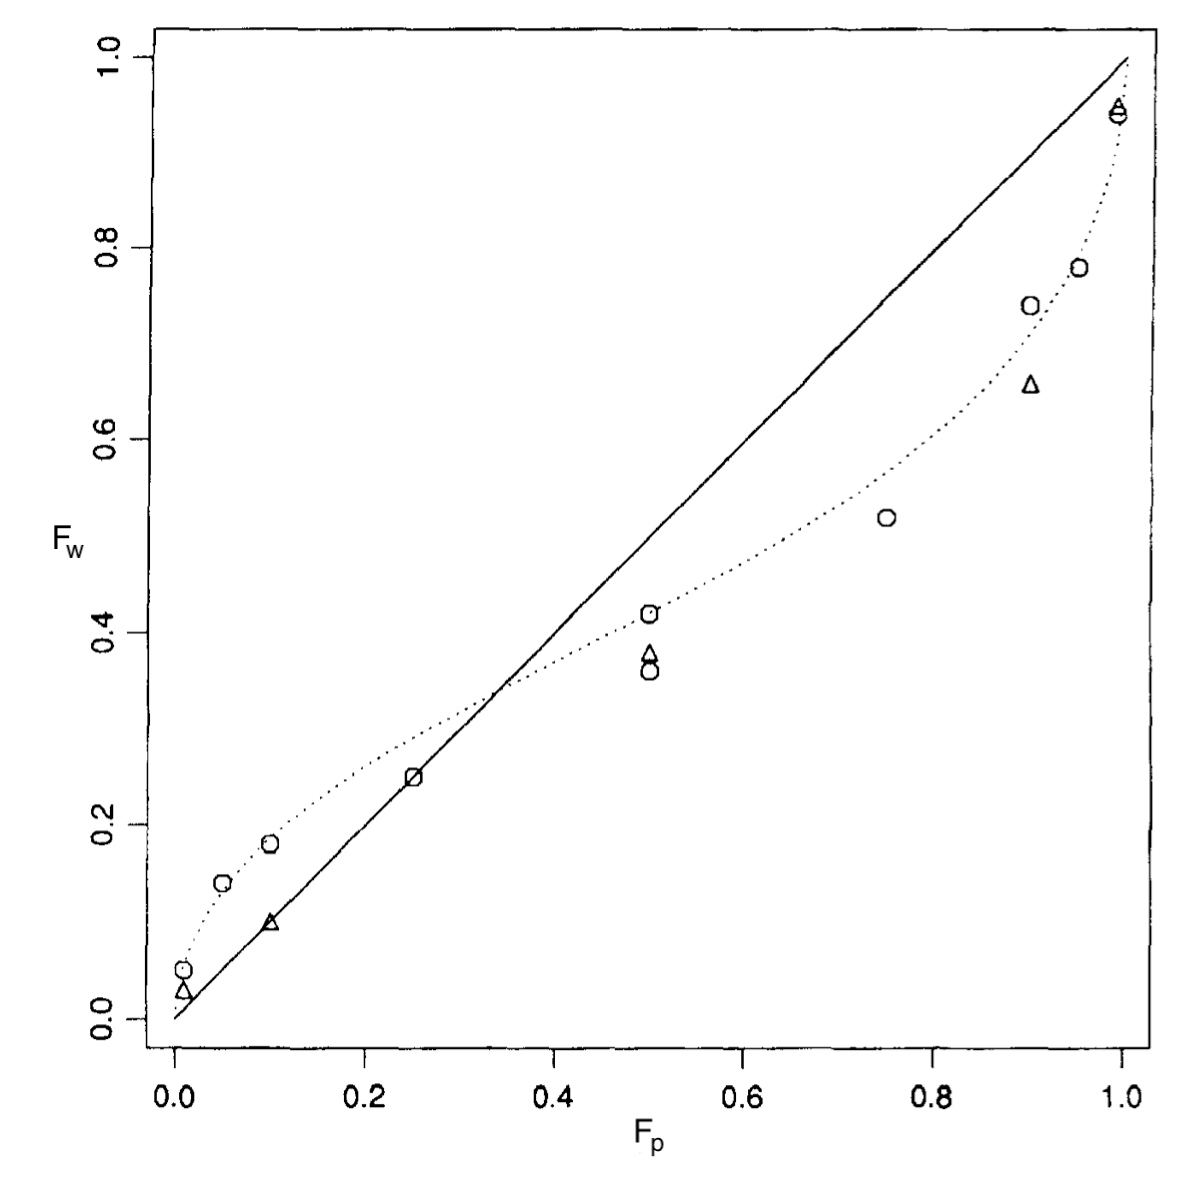
\includegraphics[width=0.5\textwidth]{./figs/TK1992.PNG}
\caption{\bsf{Empricial phenomenon of probability weighting.} Cumulative decision weights $F_w$ (used by decision makers) versus cumulative probabilities $F_p$ (used by disinterested observers), as reported by \textcite[p. 310, Fig. 1]{TverskyKahneman1992}. The figure is to be read as follows: pick a point along the horizontal axis (the probability used by a DO) and look up the corresponding value on the vertical axis of the dotted inverse-S curve (the decision weight used by a DM). For low (cumulative) probabilities (left) the decision weight exceeds the probability, and for high probabilities it's the other way around. It's the inverse-S shape of the curve that indicates this qualitative relationship.}
\flabel{TK1992}
\end{figure}

As a final piece of nomenclature, we will use the terms \textit{location} and \textit{scale} when discussing probability distributions. Consider a standard normal distribution $\ND(0,1)$ -- here, the parameters indicate location 0 and squared scale 1 (for a Gaussian that's the mean and variance). In general, for a Gaussian random variable $X$ with arbitrary  parameters for location $\mu_X$ and scale $\sigma_X$, the transformation in \eref{SN} obtains the identically-shaped location-0 and scale-1 distribution for the so standardised or normalised random variable
\be \elabel{SN}
	Z = \frac{X-\overbrace{\mu_X \mathstrut}^{\text{location}}}{\underbrace{\sigma_X\mathstrut}_{\text{scale}}}	~, \qquad \qquad Z \sim \ND(0,1)	~.
\ee
Thus the PDF of $Z$, $p(z)$ is the standard normal density with location $\mu_Z=0$ and scale $\sigma_Z=1$.

% We will show below that these observations are predicted by considerations of uncertainty about probabilities, or more generally by uncertainty about model parameters.


\section{Consistent probability weighting as a difference between models} \seclabel{ModelDiff}

Behavioural economics interprets \fref{TK1992} as evidence for a perception bias in the DM. We will keep a neutral stance. We don't consider the DO to know ``the truth'' -- he has a model of the world. Nor do we consider the DM to know ``the truth'' -- he has another model of the world. \Fref{TK1992} shows that the two models differ. Below we will go through a few generic reasons why the models may differ, and we will find that the inverse-S curve is a robust prediction in ergodicity economics -- when we emphasise that DMs have to operate along time lines.

\MK{Reference to EE falls from heaven, maybe refer to it in the intro. See TL \& discounting}

\subsection{Generic case: the Gaussian example}
Our key result is that the robust qualitative observation of the inverse-S shape in \fref{TK1992} is reproduced by assuming that the DM uses a larger scale in his model of the world than the DO. This can have numerous reasons, precaution being perhaps the most obvious one: any uncertainty the DM wishes to include in his model in addition to what the DO includes will translate into a greater scale for the DM's distribution and therefore into an inverse-S shape for any unimodal (peaked) distribution when cumulative densities are compared.

We illustrate this with a Gaussian distribution.

%\section{The Gaussian case}
%A systematic bias for decision weights to be higher than probabilities for low-probability events is a basic rule for survival. Extreme events (those of low probability) have two important properties. First, they're rare by definition; second, they're the most disruptive events. 
%
%These two facts have two consequences: first, the rarity implies that in a model fitted to observations, we will have poor statistics for such events and large uncertainty about their frequency (or ``probability''); second, because they're disruptive we have to make sure we're well prepared for them. These two facts translate into the survival rule: bias your estimates of frequencies of extreme events to be high. 
%
%To illustrate the spirit of this thought: if we think a category-5 hurricane hits once every 50-100 years, and we have to make provisions of some sort to ensure we can recover from such an event, then we have to assume the higher frequency in order to be properly prepared, \ie we have to assume the event will hit with a frequency of 1/50 p.a. Using a central value, like 1/75 p.a. would be unwise.

%We have so far established that evolution forces DMs to estimate the magnitude of noise cautiously, meaning: to err on the high side.
%As a concrete fully quantitative formal example, let's say the annual logarithmic returns, $g$, on our pension portfolio are Gaussian-distributed (yes, that may be a bad model). Let's also say we have some observations and estimate the variance of these returns to be $\sigma_1^2 \pm \sigma_2^2$. A DO without exposure to these returns would quite reasonably model them with a central best-estimate variance as $g_p \sim \ND(\mu, \sigma_1^2)$.
%
%A DM, on the other hand, would want to be on the safe side, and would assume the upper end of the range that's considered plausible for the variance. The DM would use the model $g_w \sim \ND(\mu, \sigma_1^2+\sigma_2^2$). Because the variance of the decision weights is higher than the variance of the probabilities, the decision weight corresponding to an extreme event will be higher than its probability, see \fref{probability_dists}.

Let's assume that a DO models an observable $x$ -- which will often be a future change in wealth -- as a Gaussian with location $\mu$ and variance $\sigma_1^2$. And let's further assume that a DM (for whatever reason, perhaps caution) models the same observable as a Gaussian with the same location, $\mu$, but with a greater scale, so that the variance is $\sigma_1^2+\sigma_2^2$. The DM simply assumes a broader range of plausible values, \fref{probability_dists}.

\begin{figure}[htb]
\centering
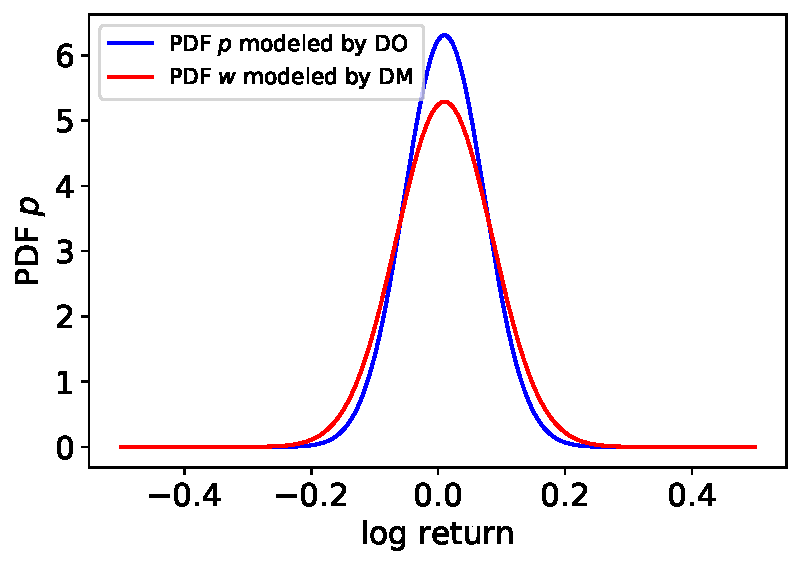
\includegraphics[width=0.7\textwidth]{./figs/probability_dists.pdf}
\caption{\bsf{Two PDFs.} Probability density function (blue), estimated by a DO; and decision-weight density function (red), estimated by a DM. The DO models returns with a best estimate for the variance and assumes the true frequency distribution is the blue line. The DM wants to be on the safe side, models returns with a greater variance, and assumes the true frequency distribution is the red line. The DM appears to the DO as someone who over-estimates probabilities of low-probability events and underestimates probabilities of high-probability events.}
\flabel{probability_dists}
\end{figure}


%\subsection{Repetition and location uncertainty}
%
%Let's stay with the investment example, and again say annual logarithmic returns are Gaussian-distributed. Let's also assume (somewhat unrealistically) that we know the variance of these returns to be $\sigma_1^2$, with certainty.
%
%Finally, we assume that the mean of the returns fluctuates. Over time, we don't always draw from the same Gaussian, but sometimes from one with a higher mean and sometimes from one with a lower mean.
%We implement this as follows: first, generate a mean, $\gamma$, from a Gaussian distribution $\gamma \sim \ND(\mu, \sigma_2^2)$. Then draw a return from a Gaussian with this mean and variance $\sigma_1^2$, meaning $g\sim\ND(\gamma,\sigma_1^2)$. Over time, the total log return is just the sum of the annual log returns, and it is equivalent to the total log return that would be generated with a Gaussian with known mean and higher variance, $g\sim \ND(\mu,\sigma_1^2+\sigma_2^2)$.
%
%Considering a single round, a DO might well use the best estimate for $\gamma$, which is $\mu$, and the known variance $\sigma_1^2$, so that $g_p\sim \ND(\mu,\sigma_1^2)$. A DM, on the other hand, who has to live with the consequences of what happens in a long sequence realizations of $g$ would use $g_w\sim \ND(\mu,\sigma_1^2+\sigma_2^2)$. Again, the situations and incentives of the DO and the DM are different, leading them to use different models (the same models as in \Secref{Survival})
%
%\section{Analysis of the Gaussian case}
%The point of the previous two sub-sections was to illustrate two different ways in which uncertainty or fluctuations in parameters lead to behaviour by a DM that leads to greater decision weights for extreme events than the probabilities a DO might assign to them. In the first case, the DO uses the best estimate, rather than a conservative estimate of the variance. In the second case, the DO assumes no fluctuations in the mean return.
%
%Both DO models give $g_p\sim\ND(\mu,\sigma_1^2)$, whereas the DM will choose the model $g_w \sim \ND(\mu,\sigma_1^2+\sigma_2^2)$.

Generically, if the DM is using a greater scale in his model, then he is using higher decision weights for low-probability events, and (because of normalisation), lower decision weights for high-probability events than the corresponding model of the DO.

%We can choose to express the DM's behaviour in terms of a mapping between the decision weights used by the DM, $w$ (red in \fref{probability_dists}), and the probabilities estimated by the DO, $p$ (blue in \fref{probability_dists}).

In the Gaussian case we can write the distributions explicitly
\be \elabel{DecisionW}
	w(x)=\frac{1}{\sqrt{2\pi (\sigma_1^2+\sigma_2^2)}}\exp\left[\frac{-(x -\mu )^2}{2 (\sigma_1^2+\sigma_2^2)}\right]
\ee
and
\be
	p(x)=\frac{1}{\sqrt{2\pi \sigma_1^2}}\exp\left[\frac{-(x -\mu )^2}{2 \sigma_1^2}\right] ~.
\elabel{p}
\ee
% 
Furthermore, we can solve \eref{p} for $(x -\mu)^2$ and substitute that in in \eref{DecisionW}. Thereby, we obtain the following expression for decision weights directly as a function of probabilities
\be
w(p)=p^{\frac{\sigma_1^2}{\sigma_1^2+\sigma_2^2}} \frac{\left(\sqrt{2\pi\sigma_1^2}\right)^{\frac{\sigma_1^2}{\sigma_1^2+\sigma_2^2}}}{\sqrt{2\pi(\sigma_1^2+\sigma_2^2)}} ~,
\elabel{w_of_p}
\ee
which we plot in \fref{probability_weights}. If we set the ratio of the DM's squared scale over the sum of the indivudal squared scales to $\alpha = \nicefrac{\sigma_1^2}{\left(\sigma_1^2 + \sigma_2^2\right)}$, we can express \eref{w_of_p} as
\be
	w(p) = p^\alpha \sqrt{\alpha\strut} \sqrt{2\pi \sigma_1^2}^{\alpha-1} . 
\ee 

\MK{Is there an interpretation to $\alpha$ or is it just a ratio? It's not the ratio of variances \ldots $\nicefrac{\sigma^2}{(\sigma_1+\sigma_2)}^2$, maybe simply the ratio of the variance and the sum of the individual variances}


\begin{figure}[htb]
\centering
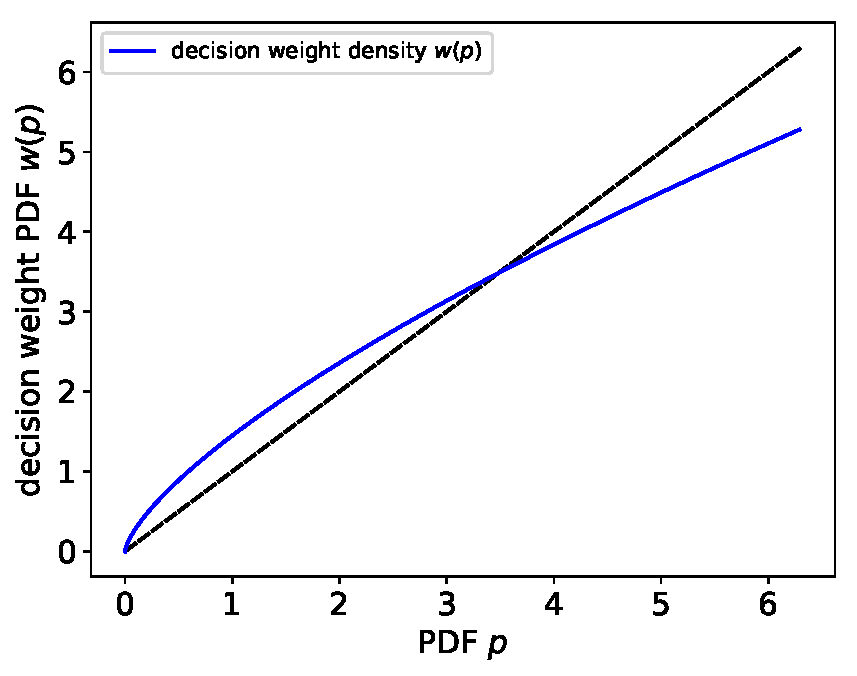
\includegraphics[width=0.7\textwidth]{./figs/decision_weights.pdf}
\caption{Decision weight density (used by a DM) vs. probability density (used by a DO) for the Gaussian model (blue), compared to the diagonal (black dashed) where DM and DO use the same parameters. For low probabilities, the decision weights are higher than the probabilities; for high probabilities they are lower.}
\flabel{probability_weights}
\end{figure}

\Fref{TwoCDFs} shows the differences in the two respective CDFs, $F_w$ and $F_p$. To produce the known probability weighting curve, we plot in \fref{subfig:GaussScale} the corresponding CDFs against each other, \ie $F_w$ against $F_p$. Whenever the DM assumes a greater scale for a unimodal distribution we find the characteristic inverse-S shape in the probability weighting curves. Thus the general mechanism does not rely on the Gaussian assumption.

%We denote these by $F_p=\int_{-\infty}^x p(s) ds$ (for the DO) and by $F_w=\int_{-\infty}^x w(s) ds$ (for the DM). 
%We will use the terms scale and location, rather than mean and standard deviation, to emphasise the generality of our arguments: 

%To clarify this nomenclature: starting with the standard form of a distribution $P(x)$ (of scale 1 and location 0), for example $P_{\text{standard}}(x)\sim \ND(0,1)$, the corresponding distributions of scale $\sigma$ and location $\mu$ are obtained by transforming $x$. With $y=\frac{x-\mu}{\sigma}$, we have $P_{\text{standard}}(y)=\ND(\mu, \sigma^2)$.

\begin{figure}[!htb]
\centering
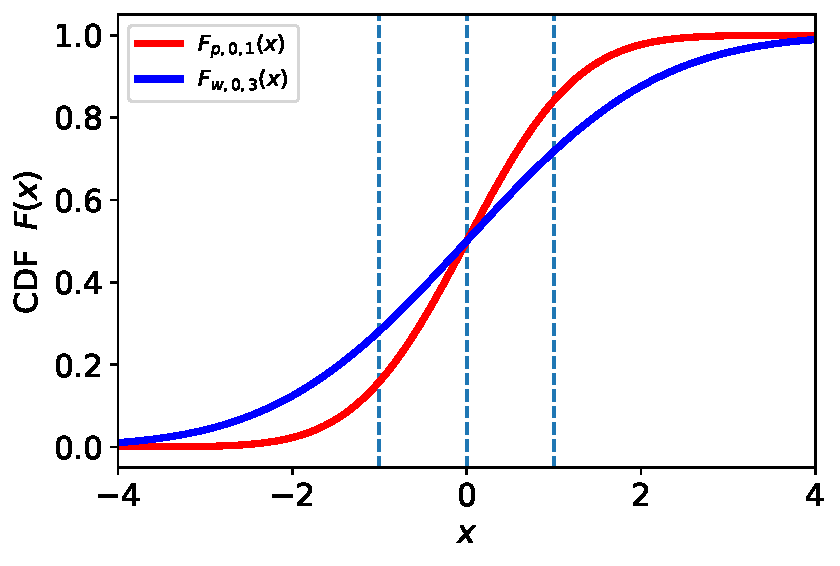
\includegraphics[width=0.7\textwidth]{./figs/TwoCDFs.pdf}
\caption{\bsf{Two Gaussian CDFs.} The DO assumes the observable $X$ follows Gaussian distribution $X \sim \ND(0,1)$, which results in the red CDF of the standard normal, $F_p(x) = \Phi_{0,1}(x)$. The DM is more cautious, in his model the same observable $X$ follows a wider Gaussian distribution with identical location, \ie a Gaussian with larger scale, $X \sim \ND(0,3)$ depicted by $F_w$ (blue). 
% 
Following the dashed vertical lines (left to right), we see that for low values of the event probability $x$ the DM's CDF is larger than the DO's CDF, $F_p(x) < F_w(x)$; the curves coincide at 0.5 because no difference in location is assumed; necessarily for large values of the event probability $x$ the DM's CDF must be lower than the DO's.}
\flabel{TwoCDFs}
\end{figure}

We have put forward the possibility that probability weighting is not a detrimental cognitive bias but an obscure way to express that DMs tend to assume a greater range of plausible outcomes than DOs. For this to be a likely explanation of the phenomenon, two conditions must be satisfied. First, there must be a reason for frequent disagreement about probabilities used in a model; second, there must be a reason for such disagreement to be consistent: there must be a relevant systematic difference between the DO and the DM. 

The first condition is satisfied because the word ``probability'' is commonly interpreted in different ways. Even once one has settled on a definition, numerical values for probabilities are still difficult to estimate from real-world observations (see \sref{tricky}).

The second condition is satisfied as follows. A DO has to build a formal model, and will include a number of sources of uncertainty in it, but often not all sources. A DM instead has to make decisions in the real world, and rules of thumb like the precautionary principle (better err on the side of caution) will often lead to extra uncertainty. For example, even if the DO may know the true probabilities of some gamble in an experiment, and builds a formal model accordingly; the DM may in addition have doubts about the DO's sincerity, or about his understanding of the rules of the game. We will return to this in \sref{condition2}.

\subsection{Lack of conceptual clarity about whose probabilities are analysed?} \seclabel{tricky}
%systematically different incentives from a real-world DM. The DO tends to have an incentive to estimate, or indeed state, probabilities as their most likely value or ``true'' value (if the DO can control the probabilities, \eg in an experiment); the DM simply strives to behave optimally under uncertainty, and that uncertainty often includes uncertainty about the probabilities or model parameters.

The conundrum surrounding the observed phenomenon of the characteristic inverse-S-shaped probability weighting vanishes if probability is understood as individual ignorance, \ie somebody's uncertainty about an observable.

\paragraph{Frequency-in-an-ensemble interpretation of probability}
It's not easy to unpack a simple probability statement like ``the probability of rain here tomorrow is 70\%.'' Tomorrow only happens once, so rain happens in 70\% of what? The technical answer to this question is usually: rain happens in 70\% of the members of an ensemble of computer simulations of what may happen tomorrow run by a weather service. So one interpretation of ``probability'' is ``relative frequency in a hypothetical ensemble of possible futures.'' 

How exactly such a statement is linked to physical reality is not completely clear. Sometimes ensembles are real, for instance, when we say the probability of having a car accident is 1\% per \SI{10000}{\km} driven -- that's a summary of statistics collected over a large ensemble of cars. In this case, it's a real ensemble that existed in the past, not an imagined one in the future. 

\paragraph{Frequency-over-time interpretation of probability}
In some situations, the statement ``70\% chance of rain tomorrow'' refers to the relative frequency over time. Before the advent of computer models in weather forecasting, people used to compare recent measurements (of wind and pressure today, say) to measurements further in the past -- weeks, months, years earlier, that were similar and where one had reason to believe that what had happened 1 day later would be similar to what will happen tomorrow.

\paragraph{Degree-of-belief interpretation of probability}
No matter how ``probability'' relates to a frequentist physical statement (whether with respect to an ensemble of simultaneous possibilities or to a time series), it also corresponds to a mental state of believing something with a degree of conviction: ``I'm 90\% sure I left my wallet in that taxi.''

Many long books have been written about the meaning of probability; for our purpose it suffices to say that there's no guarantee that a probabilistic statement will be interpreted by the listener (DM) as it was intended by whoever (DO) made the statement.

\subsubsection*{Estimation errors for probabilities}
Let's imagine the DO and DM have agreed explicitly on an interpretation of the word ``probability.'' Say they agree that they mean the relative frequency in a long time series. Real time series are, of course, of finite length. In order to estimate the relative frequency of some event in a time series, we basically count -- out of $T$ time intervals, the event $i$ occurred in $n_i$ of them, so our best estimate for the probability is $\nicefrac{n_i}{T}$. In the simplest case (and we rarely consider anything more complicated), we model the arrival of events as a Poisson process, where the standard error in the count of an event famously goes as $\sqrt{n_i}$. The standard error in the probability of an event is therefore $\nicefrac{\sqrt{n_i}}{T}$, and the relative error is $\nicefrac{1}{\sqrt{n_i}}$. Low probabilities therefore come with larger relative errors, see \tref{errors}. We note that behaviourally, it will make little difference whether a DM assigns a 0.49 probability to an event or a 0.51 probability. It will make a large difference, however, whether a DM assigns a 0.002 probability or a 0.0002 probability.

The most important message from this example is that errors in probability estimates behave differently for low probabilities than for high probabilities: absolute errors are smaller for low probabilities, but relative errors are larger for lower probabilities.

\begin{table}[!htb]
\ra{1.25}
%\small
\centering
\captionof{table}{This table assumes $T = \num{10000}$ observed time intervals. To be read as follows (first line): for an event of true probability 0.5, the most likely count in \num{10000} trials is 5000. Assuming Poisson statistics, this comes with an estimation error of $\sqrt{5000}/5000=0.01$, which is 2\% of the true probability.}\tlabel{errors}
\begin{tabular}{@{}cccc@{}}
\addlinespace
\toprule[2pt]
\makecell{Asymptotic\\(true) probability} & \makecell{Most likely\\count} & \makecell{Absolute\\estimation error} & \makecell{Relative\\estimation error}\\
\midrule[2pt]
.5 & 5000 & .01 & 2\%\\
.1 & 1000& .003 & 3\%\\
.01 & 100& .001 & 10\%\\
.001 & 10& .0003& 30\%\\
.0001 & 1& .0001 &100\%\\
\bottomrule[2pt]
\end{tabular}
\end{table}

\subsection{Disinterested observers and decision makes have different perspectives \seclabel{condition2}}
\MK{find a better section title}

The observations that led to the concept of probability weighting in prospect theory can be expressed as follows: DOs assign systematically lower weights to low-probability events than DMs.
Which of the two is wrong is unclear so long as it is unclear who means what by the word ``probability.'' Because the two types of modellers (DO and DM) pursue different goals, it may be the case that neither is wrong about the probabilities, just wrong about the goals of the other modeller.

Being a good neutral scientist, a DO has no particular interest in the success or failure of a DM. Being a good DM, the DM has every interest in his own success or failure. Throughout the history of economics, it has been a common mistake, by DOs, to assume that DMs optimise what happens to them on average in an ensemble. To the DM what happens to the ensemble is usually not a primary concern -- instead, the concern of the DM is what happens to him over time. Not distinguishing between these two perspectives is only permissible if they lead to identical predictions, and that is only the case in ergodic situations \parencite{Peters2019b}. 

It is now well known that the situation usually studied in decision theory is not ergodic in the following sense: DMs are usually observed making choices that affect their wealth, and wealth is usually modelled as a stochastic process that is not ergodic. The ensemble average of wealth does not behave like the time average of wealth.

The most striking example is the universally important case of noisy multiplicative growth -- universal because it is the fundamental process that drives evolution: noise generates the diversity (of phenotypes \ie their wealths) necessary for evolution \MK{noise generates mutations in the genotype, the noise in the world is a different animal IMO} and multiplicative growth (self-reproduction) is how successful phenotypes spread their traits in a population \MK{Covid-19 reference tempting}. This process operates on amoeba, as it does on forms of institutions, and on investment strategies.\autocite{PetersAdamou2015a}

The simplest model of noisy multiplicative growth is geometric Brownian motion, $dx=x(\mu dt+\sigma dW)$. The average over the full statistical ensemble (often studied by the DO) of geometric Brownian motion grows as $\exp(\mu t)$. The individual trajectory of geometric Brownian motion, on the other hand, grows in the long run as $\exp[(\mu-\nicefrac{\sigma^2}{2})t]$.

In the DO's ensemble perspective, noise does not affect growth and is often deemed irrelevant. In the DM's time perspective, noise reduces growth, and underestimating it would have catastrophic consequences, whereas overestimating it may lead the DM to miss out on some opportunities.

The difference between how these two perspectives evaluate the effects of noise (\ie of the probabilistic events) is qualitatively in line with the observed phenomena we set out to explain. The DM typically has large uncertainties, especially for low-probability events, and has an evolutionary incentive to err on the side of caution, \ie to behave as though low-probability (extreme) events had a higher probability than in the DO's model.

In \fref{CDF_weights} we show maps that result from the procedure illustrated in \fref{TwoCDFs}. We show separately maps that arise when the DM models the scale of the distribution differently (see \fref{subfig:GaussScale}), and when the DM models the location differently (see \fref{subfig:GaussLocation}). We then put the two together (see \fref{subfig:GaussLocScale}) and compare the result to the functional shape of $F^*_w$ which \textcite{TverskyKahneman1992} chose to fit to their observations (see \fref{subfig:PW_TK}).

Without any derivation from a physical mechanism which would motivate the specific functional form, \textcite{TverskyKahneman1992} chose to fit the following function to resemble their data\footnote{\Eref{correspondence} is the consensus functional form in the community \parencite{Barberis2013}. Whereas we provide a mechanistic explanation, psychological explanations prevail in the behavioural economics and finance literature, see \ia \textcite{WuGonzalez1996,Prelec1998,GonzalezWu1999,Stott2006,DeGiorgi2006,AbdellouiETAL2011,Wakker2010} and references especially in the latter. It remains doubtful how a psychological explanation shall compensate for a missing and/or not yet understood mechanism, generating a particular phenomenon like probability weighting.}
% 
\be
\elabel{correspondence}
F_w^*\left(F_p^*\right) = \left(F_p^*\right)^\gamma \frac{1}{\left[\left(F_p^*\right)^\gamma+\left(1-F_p^*\right)^\gamma\right]^{1/\gamma}} ~.
\ee
% 
The function 
%resembles the analytical result in that it is essentially a power law in $p_{TK}$, especially if we use $\gamma=\frac{\sigma_1^2}{\sigma_1^2+\sigma_2^2}$. It 
has only one free parameter, $\gamma$. For $\gamma=1$ both functions collapse $F_w^*\left(F_p^*\right)=F_p^*$. The function $F_w^*$ has the following property: any curvature moves the intersection with the diagonal away from the mid-point $1/2$. For this asymmetry to be reproduced in the Gaussian case, it is necessary to introduce a difference between the both the locations used by DO and DM in addition to the difference between scales (see \fref{subfig:GaussLocScale}). If we allow the possibility that the DM uses different estimates for scale and location, we can reproduce the observations in \textcite{TverskyKahneman1992} accurately, see \fref{CDF_weights}.


% \begin{figure}
% \centering
% 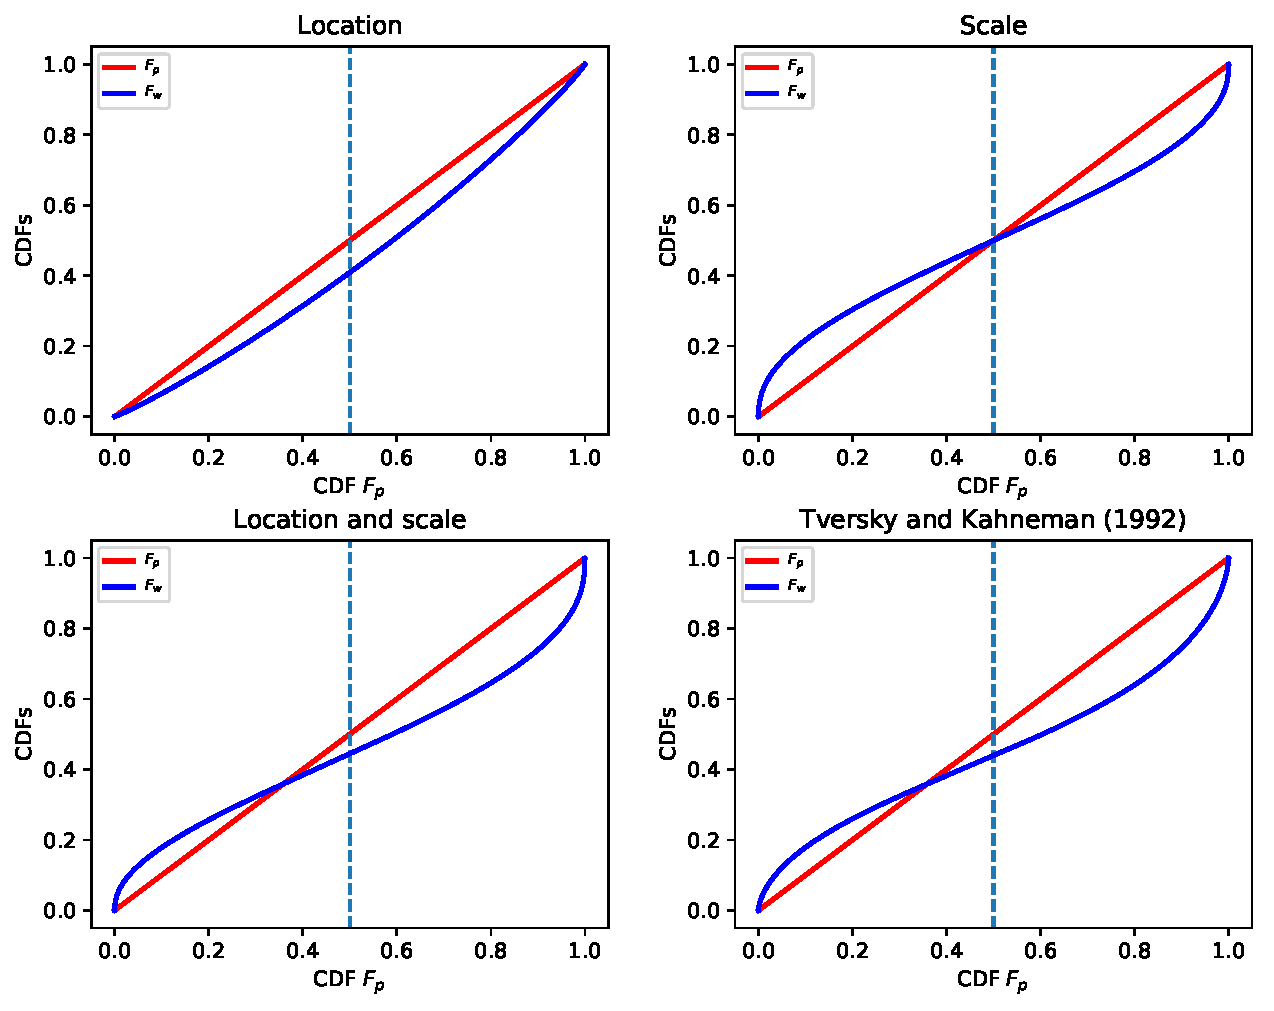
\includegraphics[width=1.0\textwidth]{./figs/Gauss_scale_location_both_KT.pdf}
% \caption{Decision weight CDFs used by a DM vs. probability CDFs used by a DO.\\ 
% Top left) Gaussian distribution, difference in scale. DO assumes location 0, scale 1; DM assumes location 0, scale 2.7 (broader than DO).\\ 
% Top right) Gaussian distribution, difference in location. DO assumes location 0, scale 1; DM assumes location 0.18 (bigger than DO), scale 1.
% Bottom left) Gaussian distribution, differences in scale and location. DO assumes location 0, scale 1; DM assumes location 0.18 (bigger than DO), scale 2.7 (broader than DO).\\ 
% Bottom right) Fit to observations reported by \textcite{TverskyKahneman1992}. This is \eref{correspondence} with $\gamma=0.65$.
% The observations by \textcite{TverskyKahneman1992} are consistent with a DM assuming a scale and location in real-world decisions that differ from those assumed by the DO.}
% \flabel{CDF_weights}
% \end{figure}

% same figure using subfigure and reps. captions 
\begin{figure}[htb]
\begin{center}
	\subcaptionbox{Gaussian distribution, difference in scale. DO assumes location 0, scale 1; DM assumes location 0, scale 2.7 (broader than DO).\flabel{subfig:GaussLocation}}
	[.45\textwidth]{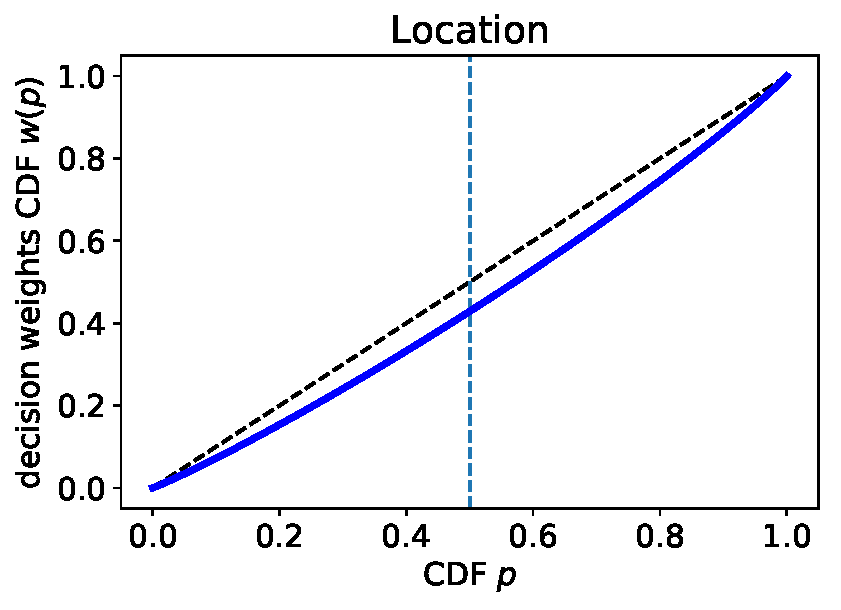
\includegraphics[width=\linewidth]{./figs/Gauss_location.pdf}}
%
	\subcaptionbox{Gaussian distribution, difference in location. DO assumes location 0, scale 1; DM assumes location 0.18 (bigger than DO), scale 1.\flabel{subfig:GaussScale}}
	[.45\textwidth]{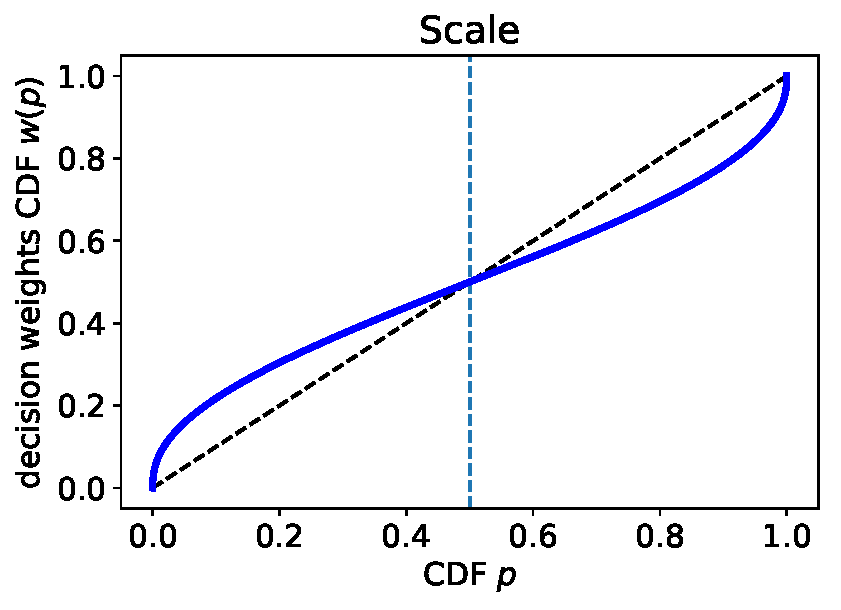
\includegraphics[width=\linewidth]{./figs/Gauss_scale.pdf}}
	\\
	\subcaptionbox{Gaussian distribution, differences in scale and location. DO assumes location 0, scale 1; DM assumes location 0.18 (bigger than DO), scale 2.7 (broader than DO).\flabel{subfig:GaussLocScale}}
	[.45\textwidth]{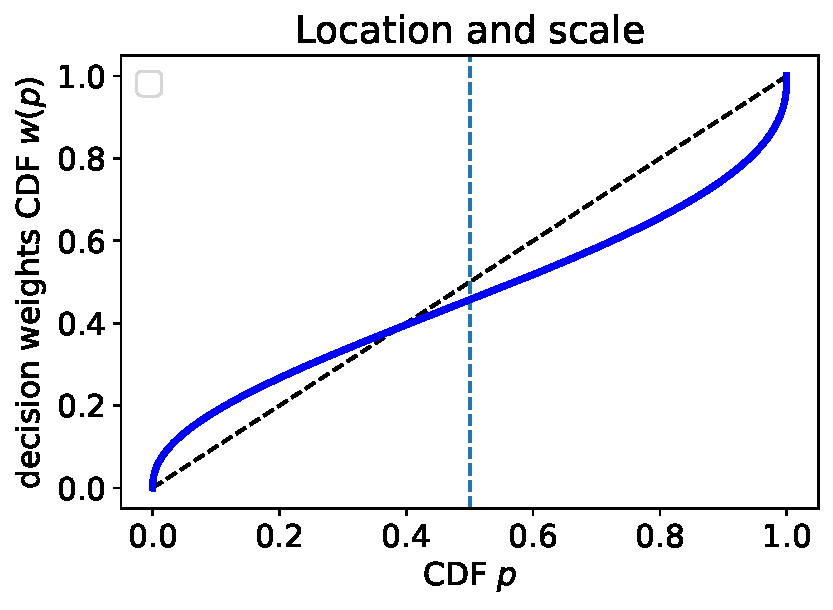
\includegraphics[width=\linewidth]{./figs/Gauss_location_and_scale.pdf}}
%
	\subcaptionbox{The observations by \textcite{TverskyKahneman1992} are consistent with a DM assuming a scale and location in real-world decisions that differ from those assumed by the DO.\flabel{subfig:PW_TK}}
	[.45\textwidth]{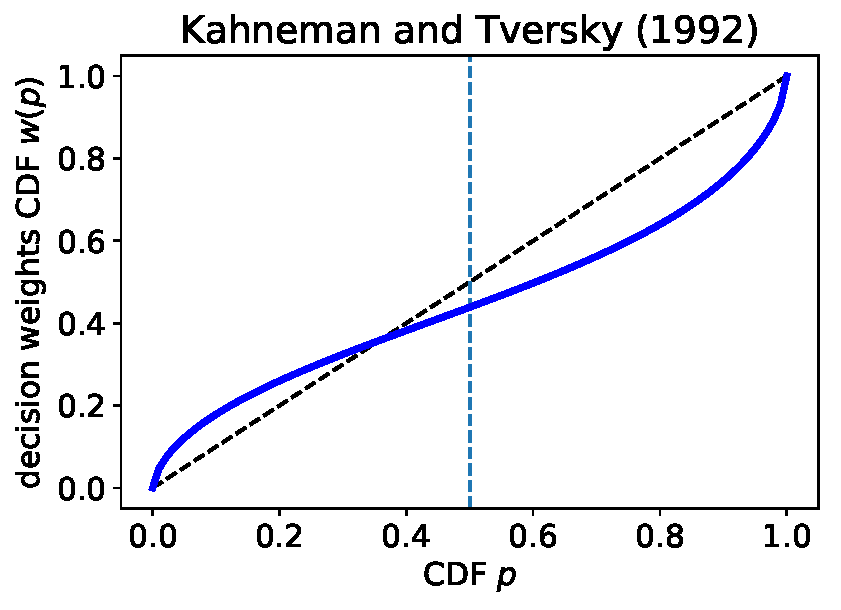
\includegraphics[width=\linewidth]{./figs/KT1992.pdf}}
% 	\vspace{1em}
\caption{\bsf{Effects of differences in location and scale for the decision weight CDFs used by a DM vs. probability CDFs used by a DO.}\\
\MK{Some more summarising text?}
% Top left) Gaussian distribution, difference in scale. DO assumes location 0, scale 1; DM assumes location 0, scale 2.7 (broader than DO).\\ 
% Top right) Gaussian distribution, difference in location. DO assumes location 0, scale 1; DM assumes location 0.18 (bigger than DO), scale 1.
% Bottom left) Gaussian distribution, differences in scale and location. DO assumes location 0, scale 1; DM assumes location 0.18 (bigger than DO), scale 2.7 (broader than DO).\\ 
% Bottom right) Fit to observations reported by \textcite{TverskyKahneman1992}. This is \eref{correspondence} with $\gamma=0.65$.
% The observations by \textcite{TverskyKahneman1992} are consistent with a DM assuming a scale and location in real-world decisions that differ from those assumed by the DO.
\flabel{CDF_weights}
\MK{Double check parameter values with py source code}
}
\end{center}
\end{figure}



\section{Other probability distributions}
Numerically, our procedure can be applied to arbitrary distributions: 
\begin{enumerate}
\item
construct a list of values for the CDF assumed by the DO, $F_p(x)$.
\item
construct a list of values for the CDF assumed by the DM, $F_w(x)$.
\item
plot $F_w(x)$ vs $F_p(x)$.
\end{enumerate}
Of course, the DM could assume a type of distribution that differs from the DO's. An infinity of combinations of assumed distributions can be explored. To illustrate the generality of the procedure, in \fref{fat_tailed_CDF} we carry it out for a (power-law tailed) Student-t distribution, where DO and DM use different shape parameters and different locations. The result is qualitatively similar to \fref{subfig:PW_TK}, corresponding to \eref{correspondence}. 

It is telling that assuming only a difference in scale and location (for the simplest Gaussian case) is already sufficient to reproduce the observations that are characterised an irrational bias and are labelled as ``probability weighting.''

\begin{figure}[htb]
\centering
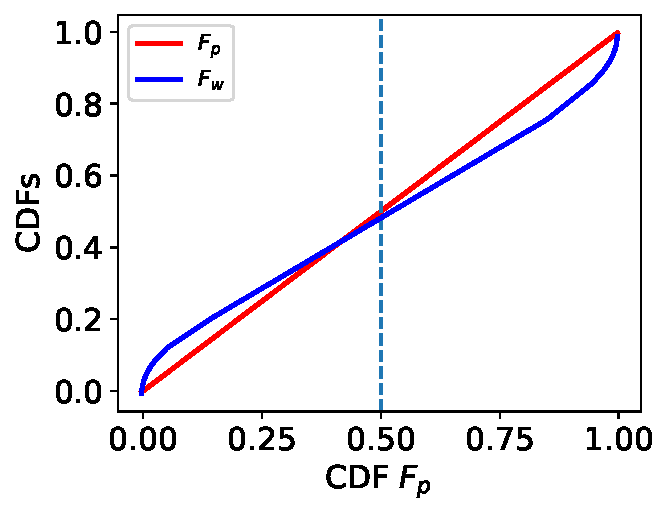
\includegraphics[width=0.7\textwidth]{./figs/Student-t.pdf}
\caption{Probability weighting for Student-t distributions, where the DM uses a different shape parameter (1) and a different location parameter (0) from those of the DO (2 and 0.2, respectively).}
\flabel{fat_tailed_CDF}
\end{figure}

\section{Conclusion/Summary}
\MK{Discuss the general action of change of measure in relation to Girsanov and risk-neutral prob measure $\mathbb{Q}$ in Math Finance?}

\MK{It has almost become custom to end with a Kacelnik quote}


\clearpage
%\bibliographystyle{humannat}
% \bibliography{./../LML_bibliography/bibliography} % name your BibTeX data base
\printbibliography

\end{document}
